\documentclass{beamer}

\usefonttheme{professionalfonts} % using non standard fonts for beamer
\usefonttheme{serif} % default family is serif

\usepackage{hyperref}
%\usepackage{minted}
\usepackage{animate}
\usepackage{graphicx}
\def\Put(#1,#2)#3{\leavevmode\makebox(0,0){\put(#1,#2){#3}}}
\usepackage{colortbl}
\usepackage{tikz}
\usepackage{amssymb}
\usepackage{enumerate}
\usepackage{arydshln}


\newcommand\blfootnote[1]{%

  \begingroup

  \renewcommand\thefootnote{}\footnote{#1}%

  \addtocounter{footnote}{-1}%

  \endgroup

}

\makeatletter

%%%%%%%%%%%%%%%%%%%%%%%%%%%%%% Textclass specific LaTeX commands.

 % this default might be overridden by plain title style

 \newcommand\makebeamertitle{\frame{\maketitle}}%

 % (ERT) argument for the TOC

 \AtBeginDocument{%

   \let\origtableofcontents=\tableofcontents

   \def\tableofcontents{\@ifnextchar[{\origtableofcontents}{\gobbletableofcontents}}

   \def\gobbletableofcontents#1{\origtableofcontents}

 }

%%%%%%%%%%%%%%%%%%%%%%%%%%%%%% User specified LaTeX commands.

\usetheme{Malmoe}

% or ...

\useoutertheme{infolines}

\addtobeamertemplate{headline}{}{\vskip2pt}

\setbeamercovered{transparent}

% or whatever (possibly just delete it)

\makeatother

\begin{document}
\title[PFLOCK report]{PFLOCK Report}
\author[AC]{Andres Calderon}
\institute[Fall'19]{University of California, Riverside}
\makebeamertitle
\newif\iflattersubsect

\AtBeginSection[] {
    \begin{frame}<beamer>
    \frametitle{Outline} 
    \tableofcontents[currentsection]  
    \end{frame}
    \lattersubsectfalse
}

\AtBeginSubsection[] {
    \begin{frame}<beamer>
    \frametitle{Outline} 
    \tableofcontents[currentsubsection]  
    \end{frame}
}

\begin{frame}{Alternative 1}
    \begin{itemize}
        \item For each partition:
        \begin{itemize}
            \item Group by Trajectory ID (\textit{tid}).
            \item Find Trajectories ID (\textit{tids}) of the neighbors of \textit{tid} in disks through timestamps (ICPE approach).
            \item Find maximal frequent patterns from \textit{tids} with $minsup=\delta$. 
        \end{itemize}

    \end{itemize}
\end{frame}

\begin{frame}{Alternative 1}
    \centering
    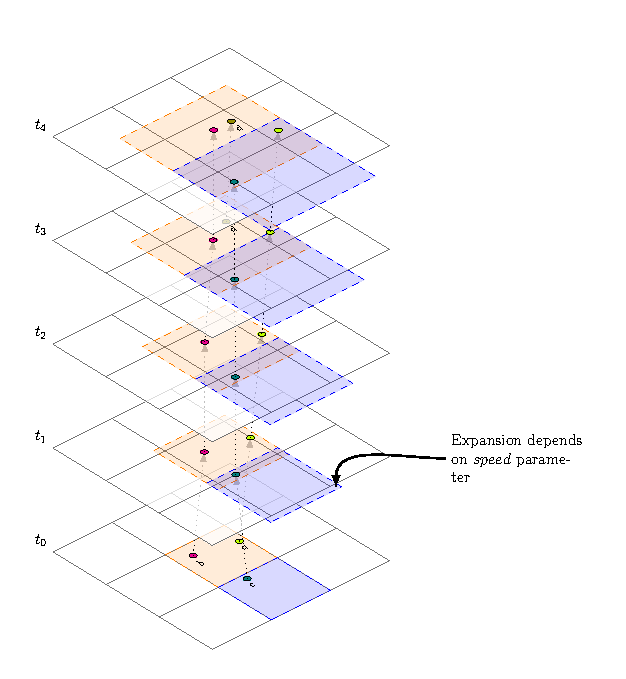
\includegraphics[height=0.95\textheight]{Figures/A1/T4}
\end{frame}

\begin{frame}{Demo 1}
    \centering
    \begin{tabular}{ l l }
        \hline
        Flock & Items \\
        \hline
        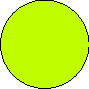
\includegraphics[scale=0.15]{Figures/lime} a	& 1 2 3	\\
        
\includegraphics[scale=0.15]{Figures/magenta} b	& 4 5	\\
        
\includegraphics[scale=0.15]{Figures/teal} c	& 6 7 8	\\
        \arrayrulecolor{black}\hline
    \end{tabular}
    \vspace{0.5cm}
    
    \scalebox{0.7}{
    \begin{tabular}{ c c l l l l l l }
        \hline
        Partition & Trajectory ID  & Neigbours & & & & & Pattern \\
        \hline
        1	& 6	& $\{7, 8\}_{t_0}$ & $\{7, 8\}_{t_1}$ & $\{7, 8\}_{t_2}$ & $\{7, 8\}_{t_3}$ & $\{7, 8\}_{t_4}$    & [7 8: 5]  \\
        \arrayrulecolor{lightgray} \hdashline
        	& 7	& $\{8\}_{t_0}$    & $\{8\}_{t_1}$    & $\{8\}_{t_2}$    & $\{8\}_{t_3}$    & $\{8\}_{t_4} $      & [8: 5]    \\
        \hdashline
        	& 8	& $\{\}_{t_0}$     &                  &                  &                  &                     &           \\
        \hline
        4	& 1	& $\{2, 3\}_{t_0}$ & $\{2, 3\}_{t_1}$ & $\{2, 3\}_{t_2}$ & $\{2, 3\}_{t_3}$ & $\{2, 3\}_{t_4} $   & [2 3: 5]  \\
        \hdashline
        	& 2	& $\{3\}_{t_0}$    & $\{3\}_{t_1}$    & $\{3\}_{t_2}$    & $\{3\}_{t_3}$    & $\{3\}_{t_4} $      & [3: 5]    \\
        \hdashline
        	& 3	& $\{\}_{t_0}$     &                  &                  &                  &                     &           \\
        \hdashline
        	& 4	& $\{5\}_{t_0}$    & $\{5\}_{t_1}$    & $\{5\}_{t_2}$    & $\{5\}_{t_3}$    & $\{5\}_{t_4} $      & [5: 5]    \\
        \hdashline
        	& 5	& $\{\}_{t_0}$     &                  &                  &                  &                     &           \\
        \arrayrulecolor{black}\hline
    \end{tabular}
    }
\end{frame}

\begin{frame}{Demo 2}
    \centering
    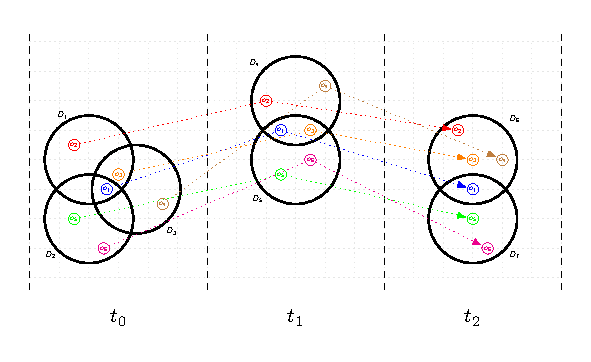
\includegraphics[height=0.8\textheight]{Figures/Trajs02}
\end{frame}

\begin{frame}{Demo 2}
    \centering
    \scalebox{0.75}{
    \begin{tabular}{ c c l l l l }
        \hline
        Partition & Trajectory ID  & Neigbours & & & Pattern \\
        \hline
        0	& 1	& $\{5, 6\}_{t_0}$ & $\{2, 3, 4\}_{t_1}$ & $\{2, 3, 4\}_{t_2}$ & [5 6: 3] \\ 
        	& 	& $\{3, 4\}_{t_0}$ & $\{3, 5, 6\}_{t_1}$ & $\{5, 6\}_{t_2}$	   & [3 4: 3] \\ 
        	& 	& $\{2, 3\}_{t_0}$ &                     &                     & [2 3: 3] \\
        \arrayrulecolor{lightgray} \hdashline
        	& 2	& $\{3\}_{t_0}$    & $\{3, 4\}_{t_1}$    & $\{3, 4\}_{t_2}$	   & [3: 3]   \\
        \hdashline
        	& 3	& $\{4\}_{t_0}$    & $\{4\}_{t_1}$       & $\{4\}_{t_2}$       & [4: 3]   \\ 
        	& 	&                  & $\{5, 6\}_{t_1}$    &                     &          \\
        \hdashline
        	& 4	& $\{\}_{t_0}$     &                     &                     &          \\
        \hdashline
        	& 5	& $\{6\}_{t_0}$    & $\{6\}_{t_1}$       & $\{6\}_{t_2}$       & [6: 3]   \\
        \hdashline
        	& 6	& $\{\}_{t_0}$     &                     &                     &          \\
        \arrayrulecolor{black}\hline
    \end{tabular}
    }
\end{frame}

\begin{frame}{What is next?}
    \begin{itemize}
        \item Check if patterns are found per row or per partition.
        \item Deal with possible redundant among partitions.
        \item Test Alternative 1 with more data.
        \item Explore Alternative 2.
    \end{itemize}
\end{frame}

\begin{frame}{Alternative 2}
    \begin{minipage}{0.5\textwidth}
        \centering
        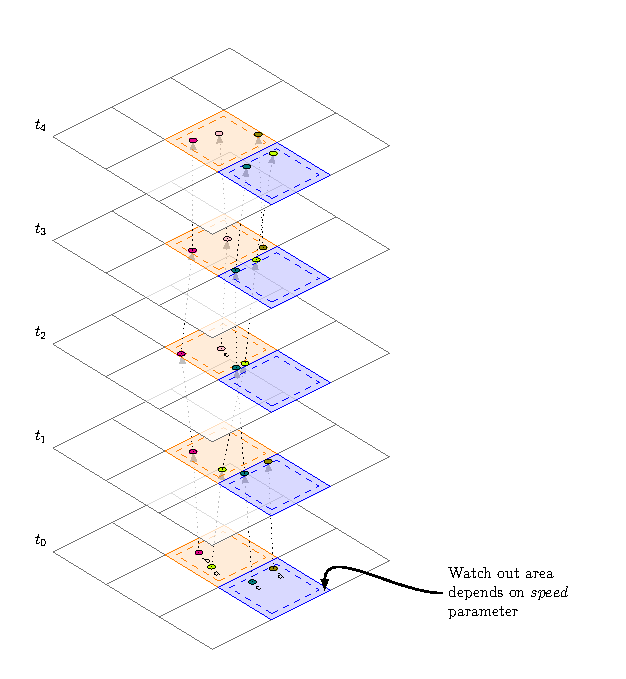
\includegraphics[width=1.25\textwidth]{Figures/A2/T4}
    \end{minipage}%
    \begin{minipage}{0.5\textwidth}
        %\centering
        \scalebox{0.7}{
        \begin{tabular}{ c c c }
            \hline
            Partition (1,1) & Partition (1, 0)  & Concat \\
            \hline
            $a_{t_0-t_2}$   & $a_{t_3-t_4}$     & $a_{t_0-t_4}\surd$    \\
            \arrayrulecolor{lightgray}\hline
            $c_{t_2-t_2}$   & $c_{t_0-t_1}$     & $c_{t_0-t_4}\surd$    \\
                            & $c_{t_3-t_4}$     &                       \\
            \hline
            $d_{t_3-t_4}$   & $a_{t_0-t_1}$     & $\times$              \\
            \arrayrulecolor{black}\hline
        \end{tabular}
        }
    \end{minipage}
\end{frame}
\end{document}
